\documentclass[border=10pt]{standalone}
\usepackage{tikz}
\usetikzlibrary{shapes,arrows,positioning,calc}
\usepackage{amsmath}

\begin{document}

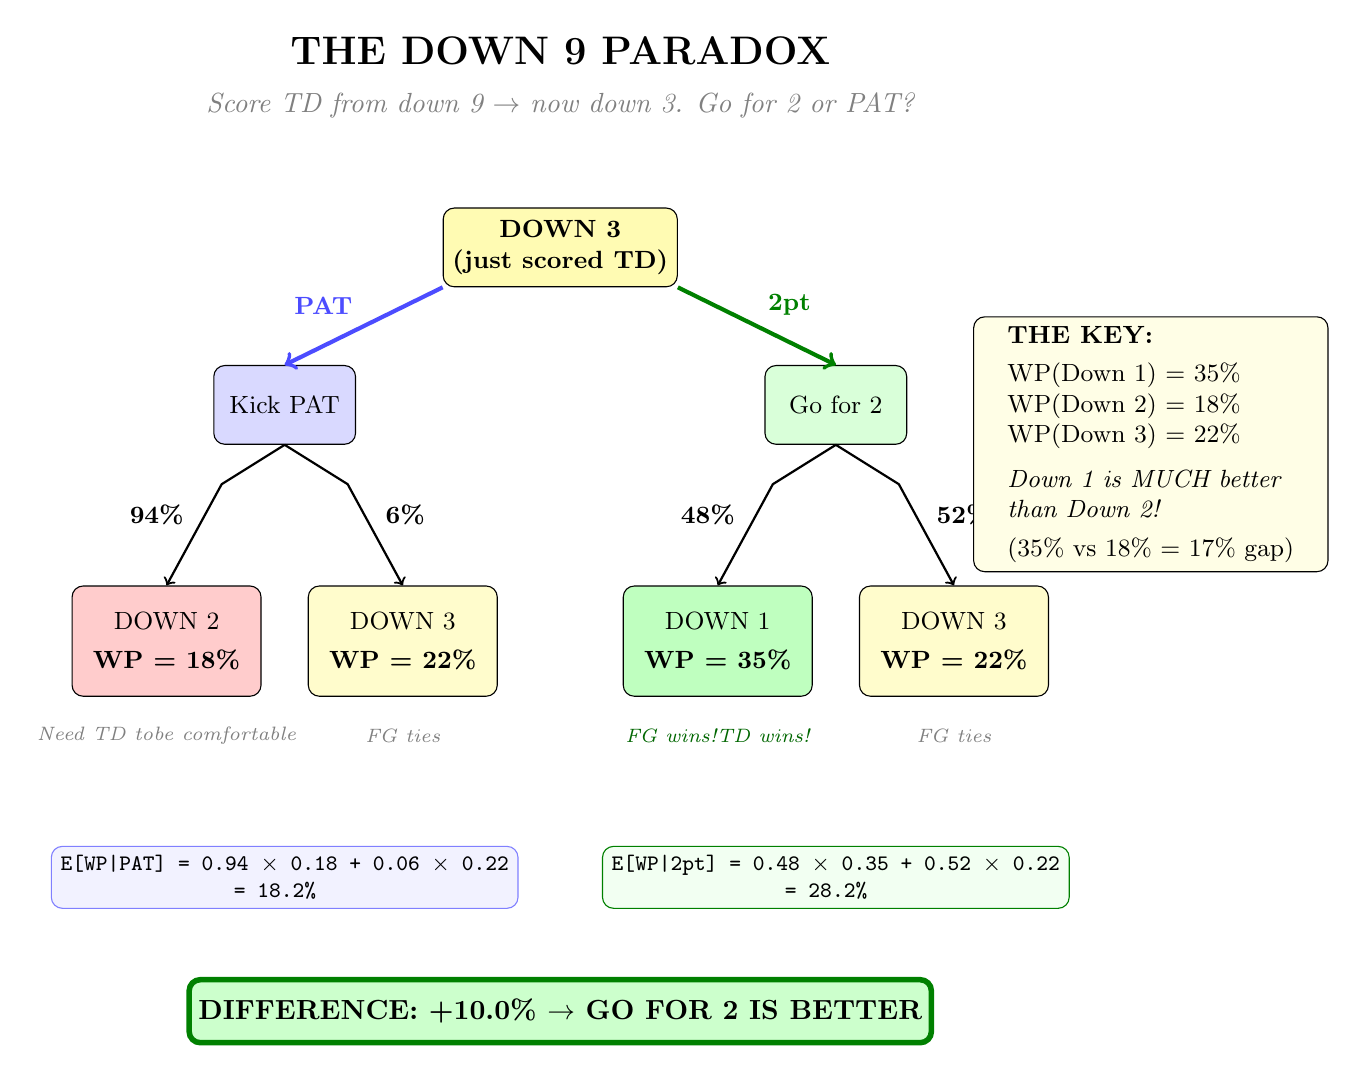
\begin{tikzpicture}[
    node distance=1.5cm,
    box/.style={rectangle, draw, rounded corners, minimum width=2.2cm, minimum height=1cm, align=center, font=\small},
    root/.style={box, fill=yellow!30, font=\small\bfseries},
    decision/.style={box, minimum width=1.8cm},
    patbox/.style={decision, fill=blue!15},
    twoptbox/.style={decision, fill=green!15},
    terminal/.style={box, minimum width=2.4cm, minimum height=1.4cm},
    down1/.style={terminal, fill=green!25},
    down2/.style={terminal, fill=red!20},
    down3/.style={terminal, fill=yellow!20},
    calcbox/.style={rectangle, draw, rounded corners, fill=white, minimum width=5.5cm, align=left, font=\footnotesize\ttfamily},
    arrow/.style={->, thick},
    prob/.style={font=\small\bfseries, midway},
    annotation/.style={font=\scriptsize\itshape, text=gray}
]

% Title
\node[font=\Large\bfseries] at (0, 5) {THE DOWN 9 PARADOX};
\node[font=\normalsize\itshape, text=gray] at (0, 4.3) {Score TD from down 9 $\to$ now down 3. Go for 2 or PAT?};

% Root node
\node[root] (root) at (0, 2.5) {DOWN 3\\(just scored TD)};

% Decision nodes
\node[patbox] (pat) at (-3.5, 0.5) {Kick PAT};
\node[twoptbox] (twopt) at (3.5, 0.5) {Go for 2};

% Arrows from root to decisions
\draw[arrow, blue!70, line width=1.5pt] (root.south west) -- (pat.north) node[prob, above left, blue!70] {PAT};
\draw[arrow, green!50!black, line width=1.5pt] (root.south east) -- (twopt.north) node[prob, above right, green!50!black] {2pt};

% Terminal nodes - PAT branch
\node[down2] (pat_make) at (-5, -2.5) {DOWN 2\\[3pt]\textbf{WP = 18\%}};
\node[down3] (pat_miss) at (-2, -2.5) {DOWN 3\\[3pt]\textbf{WP = 22\%}};

% Terminal nodes - 2pt branch
\node[down1] (twopt_make) at (2, -2.5) {DOWN 1\\[3pt]\textbf{WP = 35\%}};
\node[down3] (twopt_miss) at (5, -2.5) {DOWN 3\\[3pt]\textbf{WP = 22\%}};

% Arrows from decisions to terminals
\draw[arrow] (pat.south) -- ++(-0.8, -0.5) -- (pat_make.north) node[prob, above left] {94\%};
\draw[arrow] (pat.south) -- ++(0.8, -0.5) -- (pat_miss.north) node[prob, above right] {6\%};
\draw[arrow] (twopt.south) -- ++(-0.8, -0.5) -- (twopt_make.north) node[prob, above left] {48\%};
\draw[arrow] (twopt.south) -- ++(0.8, -0.5) -- (twopt_miss.north) node[prob, above right] {52\%};

% Annotations under terminals
\node[annotation] at (-5, -3.7) {Need TD to\\be comfortable};
\node[annotation] at (-2, -3.7) {FG ties};
\node[annotation, text=green!40!black] at (2, -3.7) {FG wins!\\TD wins!};
\node[annotation] at (5, -3.7) {FG ties};

% Calculation boxes
\node[calcbox, fill=blue!5, draw=blue!50] (calc_pat) at (-3.5, -5.5) {
E[WP|PAT] = 0.94 $\times$ 0.18 + 0.06 $\times$ 0.22\\
\hspace{2.2cm}= \textbf{18.2\%}
};

\node[calcbox, fill=green!5, draw=green!50!black] (calc_2pt) at (3.5, -5.5) {
E[WP|2pt] = 0.48 $\times$ 0.35 + 0.52 $\times$ 0.22\\
\hspace{2.2cm}= \textbf{28.2\%}
};

% Bottom line result
\node[rectangle, draw, rounded corners, fill=green!20, line width=2pt, draw=green!50!black, minimum width=8cm, minimum height=0.8cm, font=\normalsize\bfseries] at (0, -7.2) {
DIFFERENCE: +10.0\% $\to$ GO FOR 2 IS BETTER
};

% Key insight box
\node[rectangle, draw, rounded corners, fill=yellow!10, align=left, font=\small, minimum width=4.5cm] at (7.5, 0) {
\textbf{THE KEY:}\\[3pt]
WP(Down 1) = 35\%\\
WP(Down 2) = 18\%\\
WP(Down 3) = 22\%\\[5pt]
\textit{Down 1 is MUCH better}\\
\textit{than Down 2!}\\[3pt]
(35\% vs 18\% = 17\% gap)
};

\end{tikzpicture}

\end{document}
